%======================================================================
\section{Implementa\c{c}\~ao no NeoPZ e reprodu\c{c}\~ao de Rahardjo et al.\ (2007)}\label{sec:rahardjo}
%======================================================================

\begin{sloppypar}
A formula\c{c}\~ao das Se\c{c}\~oes 1--13 foi implementada no NeoPZ e aplicada aos estudos param\'etricos de
Rahardjo, Ong, Rezaur e Leong (2007), \emph{Factors controlling instability of homogeneous soil slopes under
rainfall}, J.\ Geotech.\ Geoenviron.\ Eng.\ 133(12):1532--1543. O c\'odigo \'e a vers\~ao C++ do programa Python
de refer\^encia \texttt{talude3f} (\texttt{nsat3.py}, \texttt{caso.py}) e est\'a na classe \texttt{TPZMatUnsaturatedUPwPa} (material, em \texttt{Material/Plasticity}) e no projeto
\texttt{Projects/SlopeRainfall} (problema, scripts das s\'eries, figuras e anima\c{c}\~oes).
\end{sloppypar}

\subsection{Material e an\'alise}

\begin{itemize}
\item \textbf{Inc\'ognitas e espa\c{c}os.} Deslocamento $\mathbf u$ em H1 quadr\'atico e $p_w$, $p_a$ em H1 linear
(Taylor--Hood, que satisfaz a condi\c{c}\~ao LBB, Se\c{c}\~ao 13.9), tri\^angulos em deforma\c{c}\~ao plana, regra de
3 pontos (exata para o grau 2) e mem\'oria do estado elastopl\'astico em cada ponto.
\item \textbf{Tens\~ao.} $\boldsymbol\sigma=\boldsymbol\sigma'-\alpha\,p_B\,\Id$ com
$p_B=\chi p_w+(1-\chi)p_a$; $\chi=S_w$ (Se\c{c}\~ao 3) ou $\chi$ constante. Rahardjo et al.\ usam a envolt\'oria de
Fredlund et al.\ (1978) com $\phi^b=\phi'$, isto \'e, $\chi=\tan\phi^b/\tan\phi'=1$. A tens\~ao efetiva \'e dada pelo
Mohr--Coulomb com proje\c{c}\~ao anal\'itica e tangente consistente
(\texttt{TPZPlasticStepVoigt<TPZYCMohrCoulombPV2>}), associativo ($\psi=\phi'$).
\item \textbf{Leis hidr\'aulicas} (\texttt{TPZUnsaturatedHydraulics}): reten\c{c}\~ao de Fredlund e Xing (1994) com
$C(\psi)=1$, $S_w=[\ln(e+(p_c/a)^n)]^{-m}$, ou van Genuchten (Se\c{c}\~ao 3); $k_{rw}=S_e^{\,p}$ (Leong e Rahardjo
1997) ou Mualem; $k_{ra}$ de Brooks--Corey ou Mualem, com m\'inimos $k_{rw}^{\min}$, $k_{ra}^{\min}$
(Se\c{c}\~ao 13.9).
\item \textbf{Darcy} (Se\c{c}\~ao 5) com tensor de condutividade saturada
\begin{equation}
\mathbf K=\mathbf R(\theta)\begin{bmatrix}k_1&0\\0&k_2\end{bmatrix}\mathbf R(\theta)^{\mathsf T},\qquad
\boldsymbol\lambda_w=\frac{k_{rw}}{\gamma_w}\mathbf K,\qquad
\boldsymbol\lambda_a=\frac{k_{ra}}{\gamma_w}\frac{\mu_w}{\mu_a}\mathbf K,
\end{equation}
($\theta$ = dire\c{c}\~ao de $k_1$ a partir do eixo $x$); o termo $g_a=c_a\,\mathbf q_a\cdot\nabla p_a$ do ar
(Se\c{c}\~ao 13.4) \'e mantido.
\item \textbf{Armazenamento} (Se\c{c}\~oes 7--8): $S_\pi(\alpha\Delta\varepsilon_v+\eta\Delta p_B)+nS_w\Delta p_w/K_w$
nos pontos de integra\c{c}\~ao e $n\Delta S_\pi$, $nS_a\Delta p_a/p_a^{\mathrm{abs}}$ concentrados nos v\'ertices
(forma secante conservativa $n(S^{n+1}-S^n)$; Se\c{c}\~ao 13.9). A porosidade \'e constante nos coeficientes
(fechamento de primeira ordem com $\alpha=1$ e gr\~aos incompress\'iveis, Se\c{c}\~ao 9).
\item \textbf{Newton.} Res\'iduos de Euler impl\'icito (Se\c{c}\~ao 13.7) com as equa\c{c}\~oes de massa multiplicadas
por $\Delta t$ e \textbf{jacobiano consistente completo} (inclui $\partial\lambda/\partial p$, $\partial S/\partial p$,
$\partial c_a/\partial p_a$, $\partial\chi/\partial p$ e a anisotropia); a converg\^encia quadr\'atica foi verificada
(res\'iduo das equa\c{c}\~oes de massa $5\cdot10^{-5}\to3\cdot10^{-9}\to2\cdot10^{-15}$). As condi\c{c}\~oes de
Dirichlet s\~ao eliminadas pelo filtro de equa\c{c}\~oes e o sistema \'e resolvido com Pardiso (MKL).
\item \textbf{Chuva.} Fluxo na proje\c{c}\~ao horizontal da superf\'icie com a condi\c{c}\~ao unilateral
$p_w\le0$, infiltra\c{c}\~ao $\le I_r$, complementaridade (conjunto ativo de v\'ertices alagados, como a face de
percola\c{c}\~ao da Se\c{c}\~ao~\ref{sec:barragem}); sem chuva a mesma condi\c{c}\~ao \'e uma face de percola\c{c}\~ao.
\item \textbf{Variantes} usadas na compara\c{c}\~ao: (i) \emph{modelo completo}: acoplamento hidromec\^anico e ar
ativo ($p_a=0$ s\'o na superf\'icie); (ii) \emph{ar passivo}: $p_a=0$ em todo o dom\'inio; (iii)
\emph{desacoplado com ar passivo}: os termos $S_\pi(\alpha\Delta\varepsilon_v+\eta\Delta p_B)$ s\~ao retirados das
equa\c{c}\~oes de massa (percola\c{c}\~ao em esqueleto r\'igido, como no SEEP/W); o equil\'ibrio continua usando as
press\~oes. A variante (iii) re\'une as hip\'oteses do artigo.
\end{itemize}

\subsection{Problema, par\^ametros e fator de seguran\c{c}a}

A geometria \'e a da Fig.~2 do artigo: base em $y=0$, p\'e em $y=2H_s$, crista em $y=3H_s$, plat\^os de $3H_s$ na
crista e no p\'e, face com inclina\c{c}\~ao $\alpha$; malhas de tri\^angulos do gmsh com 0,75~m at\'e 2~m de
profundidade, crescendo at\'e $0{,}3H_s$ (1684 tri\^angulos e 8874 equa\c{c}\~oes para $H_s=10$~m, $\alpha=45^\circ$;
6696 tri\^angulos e 32\,572 equa\c{c}\~oes para $H_s=40$~m). Os par\^ametros est\~ao na Tabela~\ref{tab:par}.

\begin{table}[htbp]
\centering
\caption{Par\^ametros das an\'alises (Tabela~1 do artigo e hip\'oteses de \texttt{talude3f}).}\label{tab:par}
\small
\begin{tabular}{p{3.6cm}p{8.6cm}l}
\toprule
Grandeza & Valor & Origem\\
\midrule
Solos $f_{10,-4}$, $f_{50,-5}$, $f_{100,-6}$ & $a=10$, 50, 100~kPa; $k_s=10^{-4}$, $10^{-5}$, $10^{-6}$~m/s & artigo\\
Reten\c{c}\~ao e $k_{rw}$ & Fredlund--Xing $n=m=1$, $\theta_s=0{,}45$; $k_w=k_s\Theta^4$ & artigo\\
Resist\^encia & $c'=10$~kPa, $\phi'=\phi^b=26^\circ$ ($\chi=1$), $\gamma=20$~kN/m$^3$ & artigo\\
Condi\c{c}\~ao inicial & NA a $H_w$ abaixo do p\'e, inclinado de $7^\circ$; suc\c{c}\~ao $\le75$~kPa & artigo\\
Chuva & $I_r$ durante 24~h; 48~h simuladas (240~h na S\'erie A) & artigo\\
Elasticidade, dilat\^ancia & $E=20$~MPa, $\nu=0{,}3$, $\psi=\phi'$ & hip\'otese\\
Ar & Brooks--Corey $\lambda=3$, $k_{ra}^{\min}=10^{-4}$, $\mu_w/\mu_a=55{,}6$, g\'as ideal & hip\'otese\\
\'Agua & $K_w=2{,}2$~GPa, $\gamma_w=9{,}81$~kN/m$^3$ & hip\'otese\\
Passos de tempo & 15~min na chuva, 1~h nas 24~h seguintes, 4~h depois; bissec\c{c}\~ao & \texttt{talude3f}\\
\bottomrule
\end{tabular}
\end{table}

Contornos: base fixa e laterais em rolete; carga total imposta nas laterais abaixo do NA; base e laterais acima do
NA imperme\'aveis; $p_a=0$ na superf\'icie. O estado inicial \'e o peso pr\'oprio aplicado em 4 incrementos com as
press\~oes congeladas, seguido de $\mathbf u=\mathbf 0$ com $\boldsymbol\sigma'$ mantida.

O artigo calcula o FS por Bishop simplificado (SLOPE/W) com as poropress\~oes de cada instante. Aqui, em cada
instante, faz-se uma an\'alise independente com $p_w$ e $p_a$ congeladas (o material assembla s\'o o equil\'ibrio) e a
mem\'oria do transiente \'e restaurada depois:
\begin{itemize}
\item \textbf{Redu\c{c}\~ao de resist\^encia (SRM)}: estado geost\'atico com $c'/F_0$, $\tan\phi'/F_0$
($F_0=0{,}6$, para encontrar FS $<1$) e aumento de $F$ at\'e a perda de converg\^encia (bissec\c{c}\~ao at\'e 0,01). \'E
o FS comparado com o do artigo.
\item \textbf{Aumento da gravidade (GI)}: a partir do estado sem peso, $\lambda$ multiplica o peso do solo e a parte
positiva de $p_B$; a suc\c{c}\~ao \'e mantida (multiplic\'a-la por $\lambda$ faria a resist\^encia crescer com o peso e
o talude nunca romperia).
\end{itemize}

Foram calculados 144 casos: S\'eries A (36), B (21, nas tr\^es variantes), C (15) e D (12), e 18 casos de
anisotropia. O tempo m\'edio por caso de 48~h foi de 13--26~min com $H_s=10$~m (um n\'ucleo) e cerca de 4~h com
$H_s=40$~m.

\subsection{Fator de seguran\c{c}a inicial}

O FS inicial coincide com o do artigo em todas as geometrias (Tabela~\ref{tab:fsini}), o que valida a geometria, o
estado inicial, a tens\~ao de Bishop e a an\'alise de estabilidade por elementos finitos.

\begin{table}[htbp]
\centering
\caption{FS inicial: NeoPZ (SRM) e Rahardjo et al.\ (2007).}\label{tab:fsini}
\begin{tabular}{lcccc}
\toprule
S\'erie A ($H_s=10$, $H_w=5$~m), $\alpha$ & $26{,}6^\circ$ & $33{,}7^\circ$ & $45^\circ$ & $63{,}4^\circ$\\
NeoPZ & 2,547 & 2,350 & 2,119 & 1,775\\
Tabela 7 ($3{,}153-0{,}023\alpha$) & 2,54 & 2,38 & 2,12 & 1,69\\
\midrule
S\'erie D ($\alpha=45^\circ$, $H_w=5$~m), $H_s$ & 5~m & 10~m & 20~m & 40~m\\
NeoPZ & 3,211 & 2,119 & 1,488 & 1,125\\
Fig.~10 & 3,22 & 2,11 & 1,50 & 1,12\\
\bottomrule
\end{tabular}

\vspace{6pt}
\begin{tabular}{lccccc}
\toprule
S\'erie C ($H_s=10$~m, $\alpha=45^\circ$), $H_w$ & 2,5~m & 5~m & 7,5~m & 10~m & 15~m\\
NeoPZ & 1,800 & 2,119 & 2,350 & 2,397 & 2,397\\
Fig.~8 & 1,80 & 2,11 & 2,33 & 2,35 & 2,35\\
\bottomrule
\end{tabular}
\end{table}

\subsection{S\'erie B: intensidade da chuva}

A Fig.~\ref{fig:Bvar} e a Tabela~\ref{tab:B} comparam o FS m\'inimo das tr\^es variantes com a sigmoide da Eq.~6 do
artigo, $F_{s(\min)}=A+B/(1+e^{-(I_r-C)/D})$, e a Tabela~\ref{tab:fig5b} compara a evolu\c{c}\~ao no tempo com a
Fig.~5b. As Figs.~\ref{fig:Bdesac} e \ref{fig:Bcomp} mostram as curvas FS($t$) da variante com as hip\'oteses do
artigo e do modelo completo.

\begin{figure}[htbp]
\centering
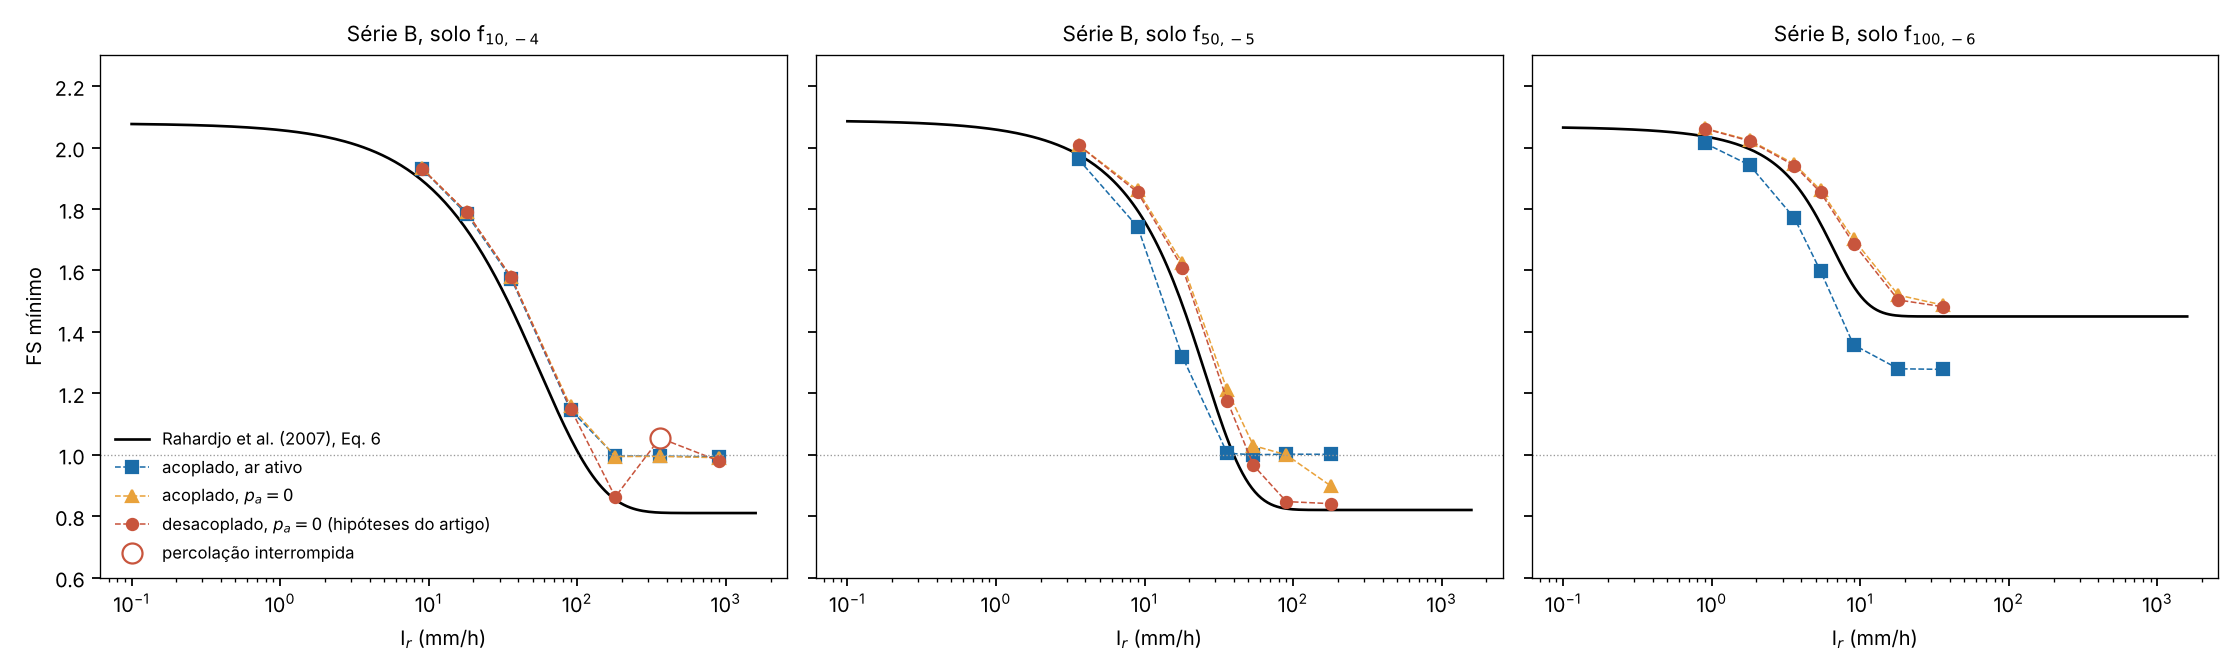
\includegraphics[width=\textwidth]{figuras/B_variantes_fsmin.png}
\caption{S\'erie B ($H_s=10$~m, $\alpha=45^\circ$, $H_w=5$~m, 24~h de chuva): FS m\'inimo $\times$ $I_r$ nas tr\^es
variantes do modelo e Eq.~6 do artigo (ajuste aos seus resultados, Fig.~7). C\'irculo vazado: percola\c{c}\~ao
interrompida antes do fim da chuva (m\'inimo superestimado).}\label{fig:Bvar}
\end{figure}

\begin{table}[htbp]
\centering
\caption{S\'erie B: FS m\'inimo. Eq.~6: ajuste do artigo; (i) modelo completo; (ii) ar passivo; (iii) desacoplado
com ar passivo (hip\'oteses do artigo). $^*$Percola\c{c}\~ao interrompida \`as 8,5~h (superf\'icie toda alagada).}
\label{tab:B}
\begin{tabular}{llcccc}
\toprule
Solo & $I_r$ (mm/h) & Eq.~6 & (i) completo & (ii) ar passivo & (iii) desacoplado\\
\midrule
$f_{10,-4}$ & 9 & 1,89 & 1,93 & 1,93 & 1,93\\
 & 36 & 1,48 & 1,57 & 1,58 & 1,58\\
 & 90 & 1,05 & 1,15 & 1,16 & 1,15\\
 & 180 & 0,85 & 1,00 & 0,99 & \textbf{0,86}\\
 & 360 & 0,81 & 1,00 & 1,00 & 1,05$^*$\\
 & 900 & 0,81 & 0,99 & 0,99 & 0,98$^*$\\
\midrule
$f_{50,-5}$ & 3,6 & 1,98 & 1,96 & 2,01 & 2,01\\
 & 9 & 1,79 & 1,74 & 1,86 & 1,85\\
 & 18 & 1,49 & 1,32 & 1,62 & 1,61\\
 & 36 & 1,05 & 1,01 & 1,21 & 1,18\\
 & 54 & 0,89 & 1,00 & 1,03 & \textbf{0,97}\\
 & 90 & 0,82 & 1,00 & 1,00 & \textbf{0,85}\\
 & 180 & 0,82 & 1,00 & 0,90 & \textbf{0,84}\\
\midrule
$f_{100,-6}$ & 0,9 & 2,04 & 2,01 & 2,06 & 2,06\\
 & 3,6 & 1,88 & 1,77 & 1,95 & 1,94\\
 & 9 & 1,55 & 1,36 & 1,70 & 1,69\\
 & 18 & 1,45 & 1,28 & 1,52 & 1,50\\
 & 36 & 1,45 & 1,28 & 1,49 & 1,48\\
\bottomrule
\end{tabular}
\end{table}

\begin{table}[htbp]
\centering
\caption{Solo $f_{50,-5}$: FS ao longo do tempo, Fig.~5b do artigo (digitalizada, $\pm0{,}03$) e NeoPZ
(modelo completo / desacoplado com ar passivo).}\label{tab:fig5b}
\begin{tabular}{lcccc}
\toprule
$I_r$ (mm/h) & $t=6$~h & $t=12$~h & $t=24$~h & $t=48$~h\\
\midrule
9 & 2,00 / 2,00 / 2,03 & 1,92 / 1,90 / 1,96 & 1,78 / 1,74 / 1,85 & 1,85 / 1,87 / 1,91\\
18 & 1,92 / 1,88 / 1,96 & 1,76 / 1,67 / 1,83 & 1,50 / 1,32 / 1,61 & 1,60 / 1,65 / 1,68\\
36 & 1,72 / 1,61 / 1,82 & 1,40 / 1,18 / 1,56 & 1,04 / 1,00 / 1,18 & 1,24 / 1,51 / 1,33\\
54 & 1,49 / 1,36 / 1,67 & 1,20 / 1,08 / 1,32 & 0,90 / 1,00 / 0,97 & 1,15 / 1,51 / 1,19\\
90 & 1,35 / 1,24 / 1,44 & 1,18 / 1,06 / 1,19 & 0,86 / 1,00 / 0,85 & 1,15 / 1,51 / 1,17\\
180 & 1,33 / 1,20 / 1,37 & 1,14 / 1,06 / 1,16 & 0,82 / 1,00 / 0,84 & 1,15 / 1,52 / 1,17\\
\bottomrule
\end{tabular}
\end{table}

\begin{figure}[htbp]
\centering
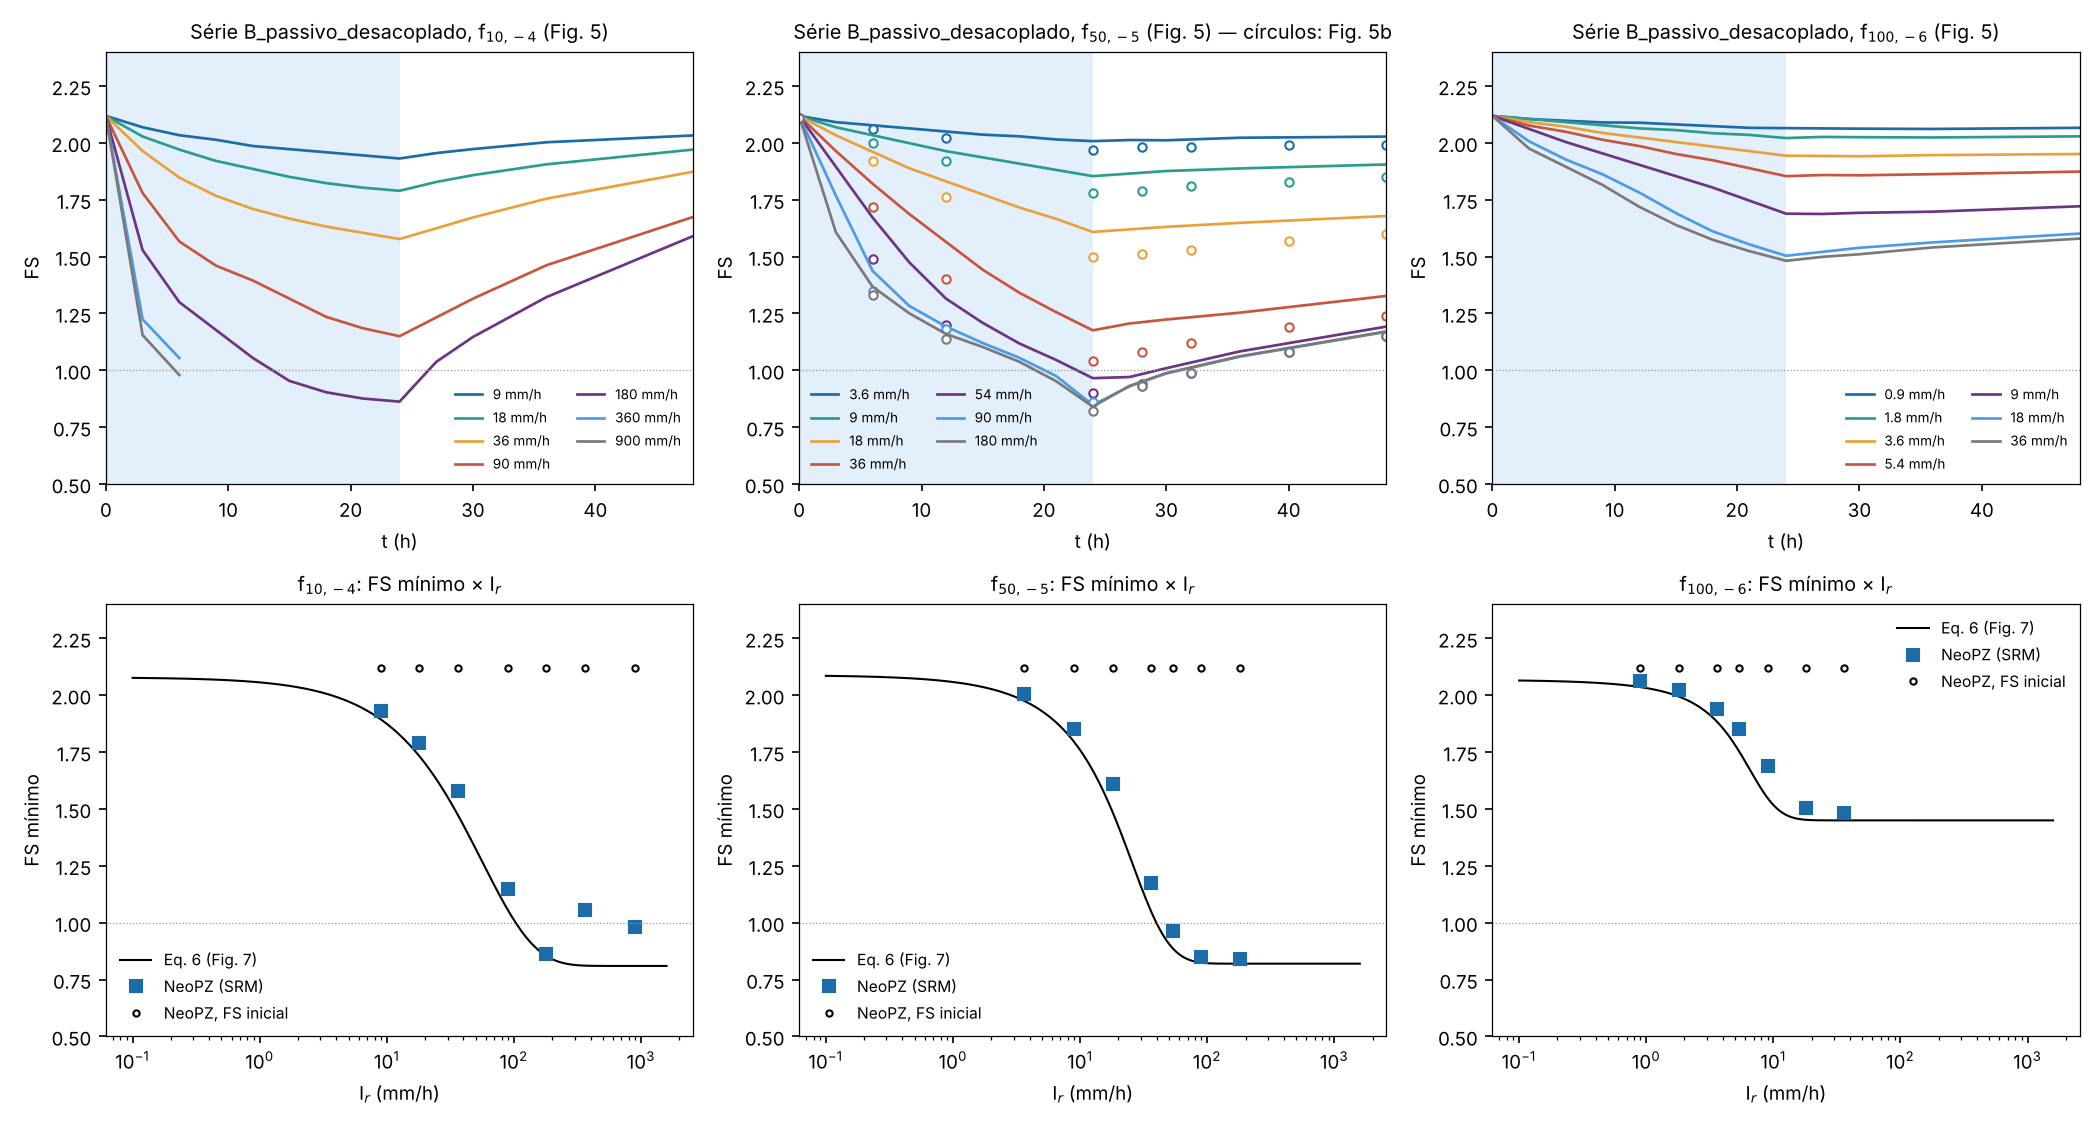
\includegraphics[width=\textwidth]{figuras/B_passivo_desacoplado_fs.png}
\caption{S\'erie B, desacoplado com ar passivo (hip\'oteses do artigo). Acima: FS($t$) (c\'irculos: Fig.~5b); abaixo:
FS m\'inimo $\times$ $I_r$ e Eq.~6.}\label{fig:Bdesac}
\end{figure}

\begin{figure}[htbp]
\centering
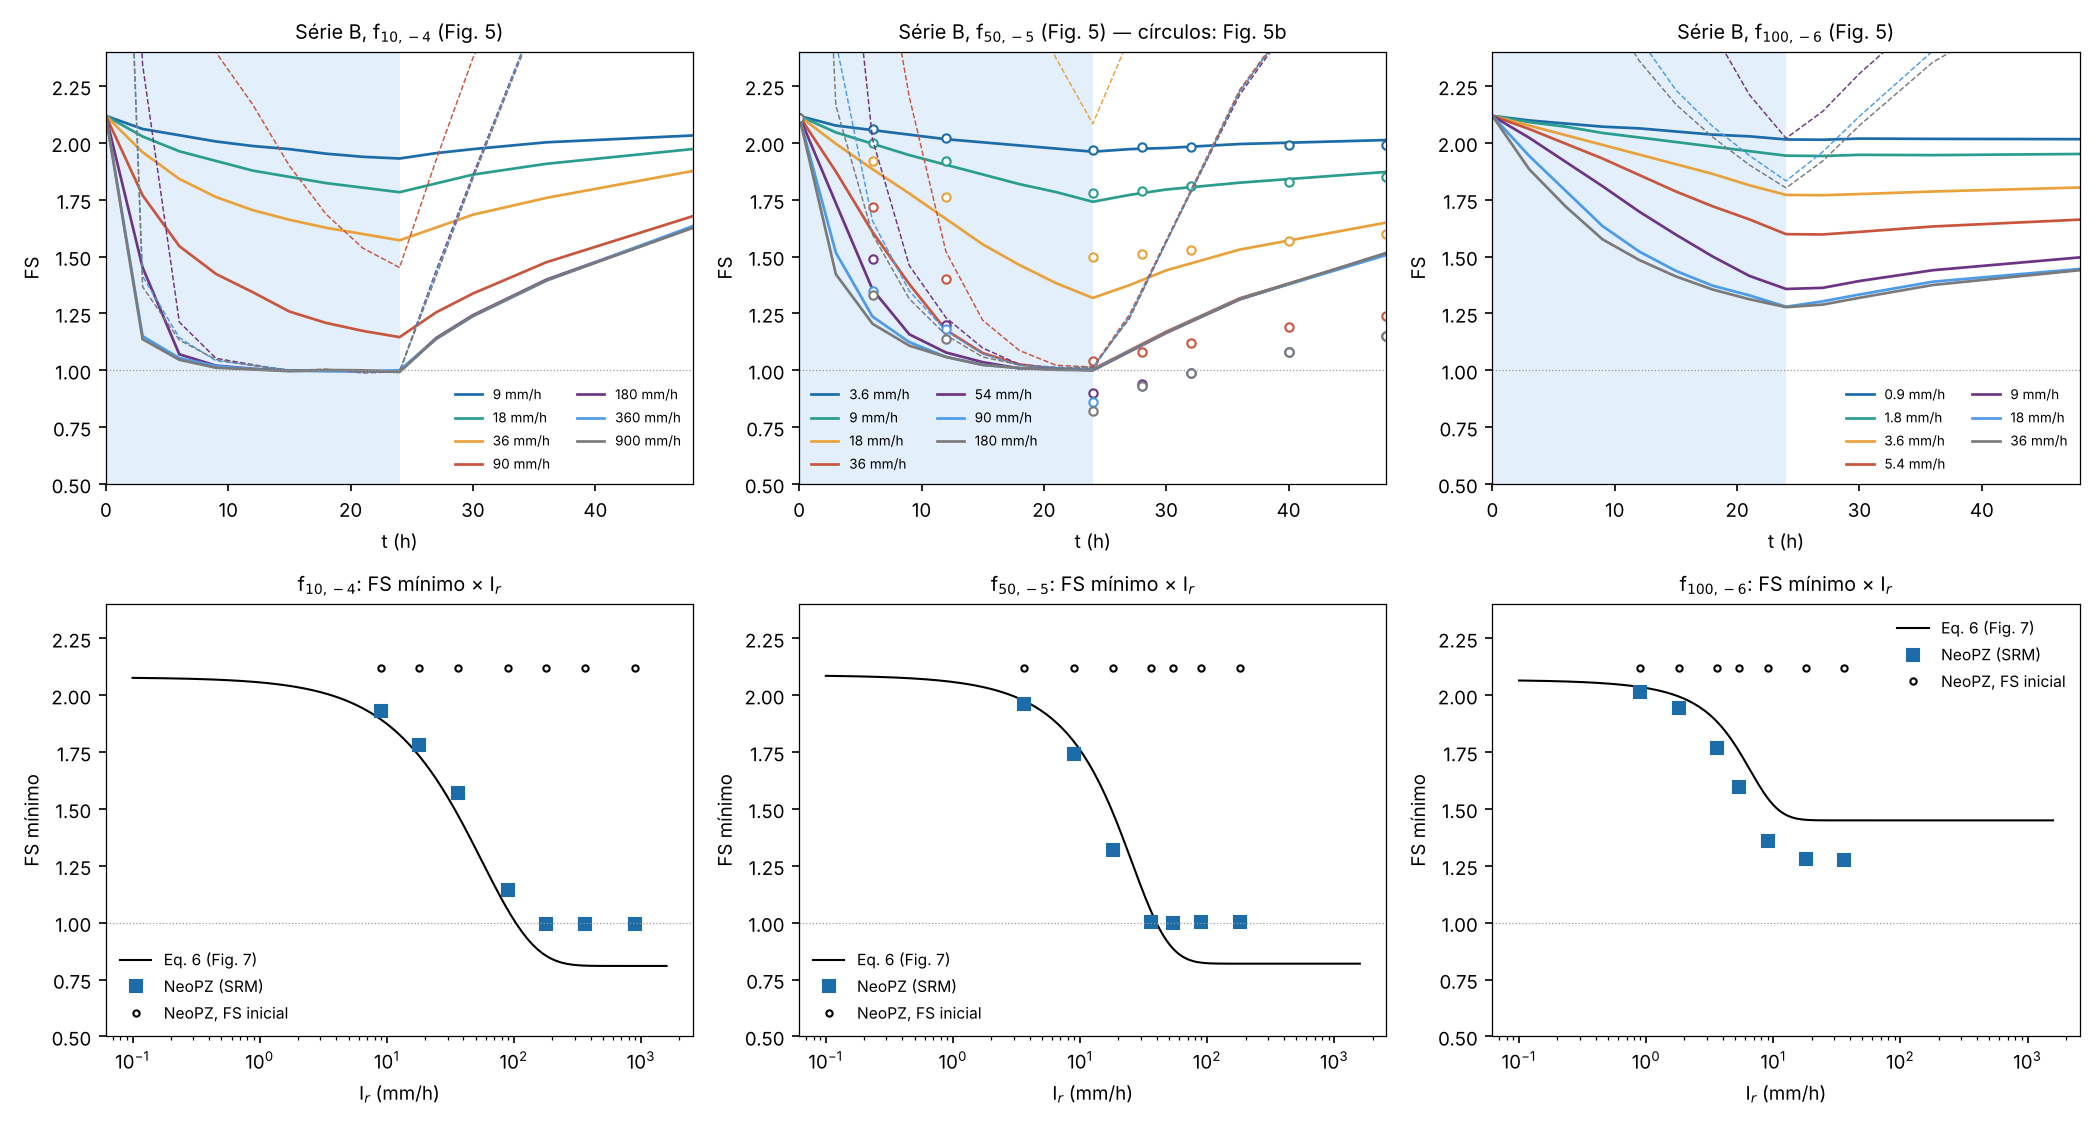
\includegraphics[width=\textwidth]{figuras/B_fs.png}
\caption{S\'erie B, modelo completo (acoplado, ar ativo). Linhas tracejadas: FS por aumento da gravidade.}
\label{fig:Bcomp}
\end{figure}

Observa\c{c}\~oes:
\begin{enumerate}
\item \textbf{Com as hip\'oteses do artigo} (variante iii) o FS m\'inimo segue a sigmoide da Eq.~6 nos tr\^es solos,
inclusive o patamar inferior (0,84--0,86 contra 0,81--0,82) e a recupera\c{c}\~ao depois da chuva da Fig.~5b. As
diferen\c{c}as restantes (FS 0,05--0,15 maior nas chuvas moderadas) s\~ao compat\'iveis com SRM $\times$ Bishop e com a
digitaliza\c{c}\~ao.
\item \textbf{No modelo completo o FS n\~ao desce abaixo de $\approx1{,}00$.} O transiente acoplado nunca perde o
equil\'ibrio: com Mohr--Coulomb associativo a plastifica\c{c}\~ao dilata o solo e, com o acoplamento
$S_w\alpha\,\dot\varepsilon_v$, a dilata\c{c}\~ao reduz $p_w$ (gera suc\c{c}\~ao) e aumenta a resist\^encia: o talude
estabiliza no limite. O mesmo patamar aparece nas S\'eries A, C e D. A recupera\c{c}\~ao depois da chuva \'e mais r\'apida
(FS 1,51 em 48~h contra 1,24).
\item \textbf{O ar ativo reduz o FS nos solos pouco perme\'aveis} ($f_{100}$ com 18~mm/h: 1,28 contra 1,50 com
$p_a=0$; $f_{50}$ com 18~mm/h: 1,32 contra 1,62). O ar aprisionado sob a frente de umedecimento chega a 50~kPa
(Fig.~\ref{fig:campos}) e eleva $p_w$ (positiva sob a crista, com suc\c{c}\~ao ainda positiva); com $\chi=1$ a
tens\~ao efetiva depende de $p_w$.
\item O FS por aumento da gravidade \'e muito maior que o SRM no estado inicial (5,7 contra 2,1), porque a suc\c{c}\~ao
mantida \'e uma parcela de resist\^encia que n\~ao cresce com o peso; os dois coincidem perto da ruptura
(Fig.~\ref{fig:fstempo}).
\end{enumerate}

\begin{figure}[htbp]
\centering
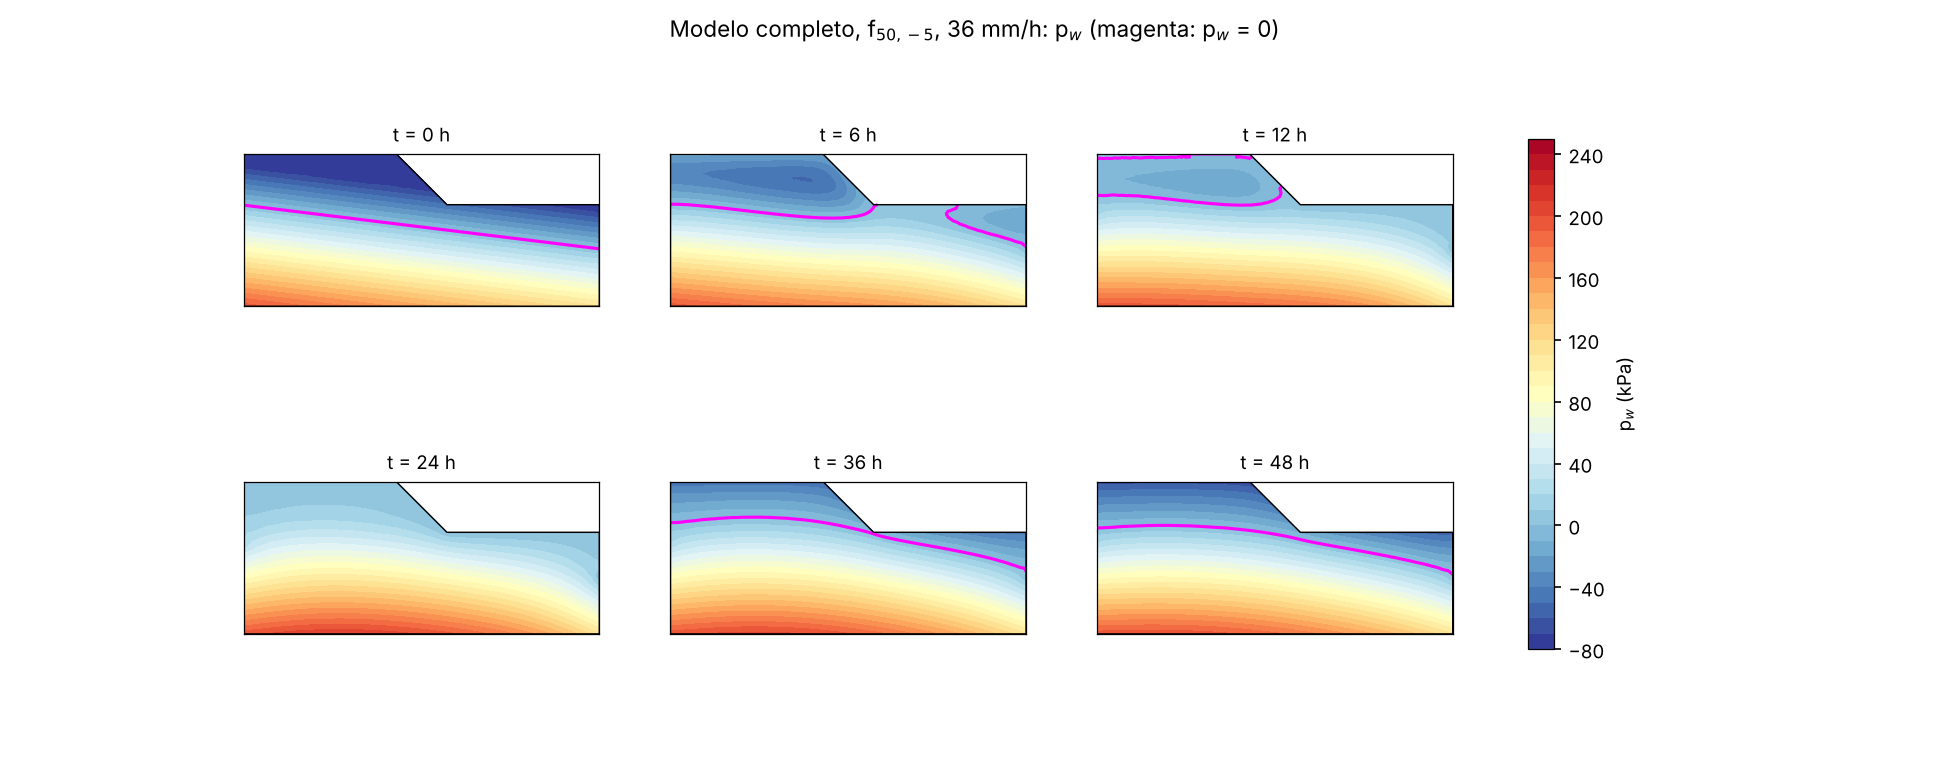
\includegraphics[width=0.95\textwidth]{figuras/campos_pw_f50_a45_H10_Hw5_I36_B.png}\\
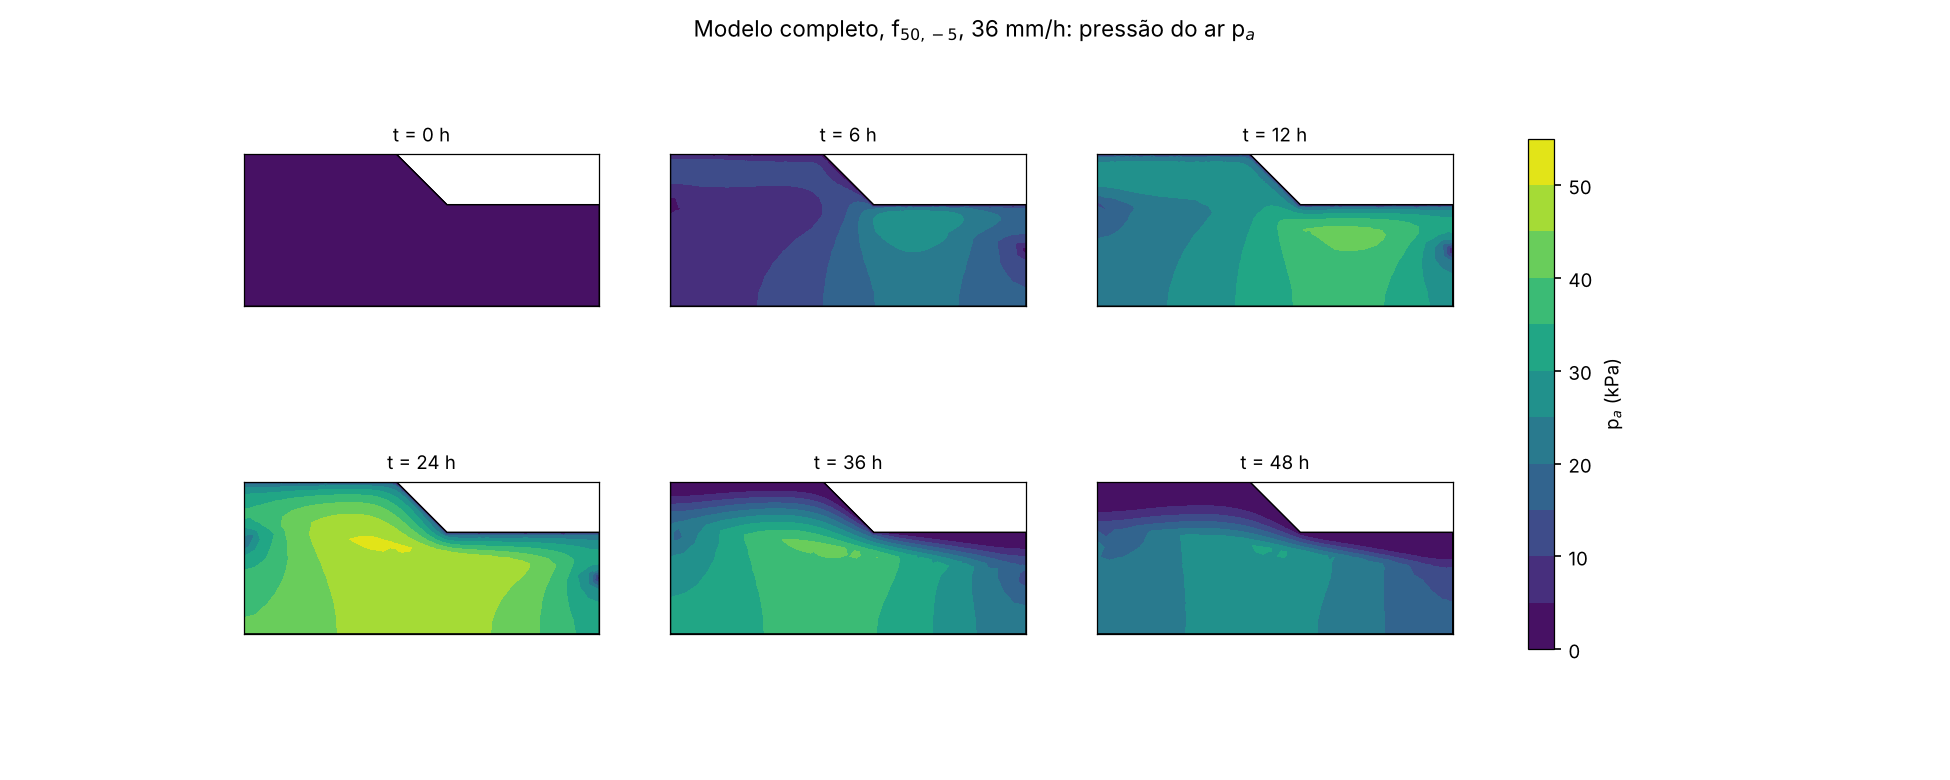
\includegraphics[width=0.95\textwidth]{figuras/campos_pa_f50_a45_H10_Hw5_I36_B.png}\\
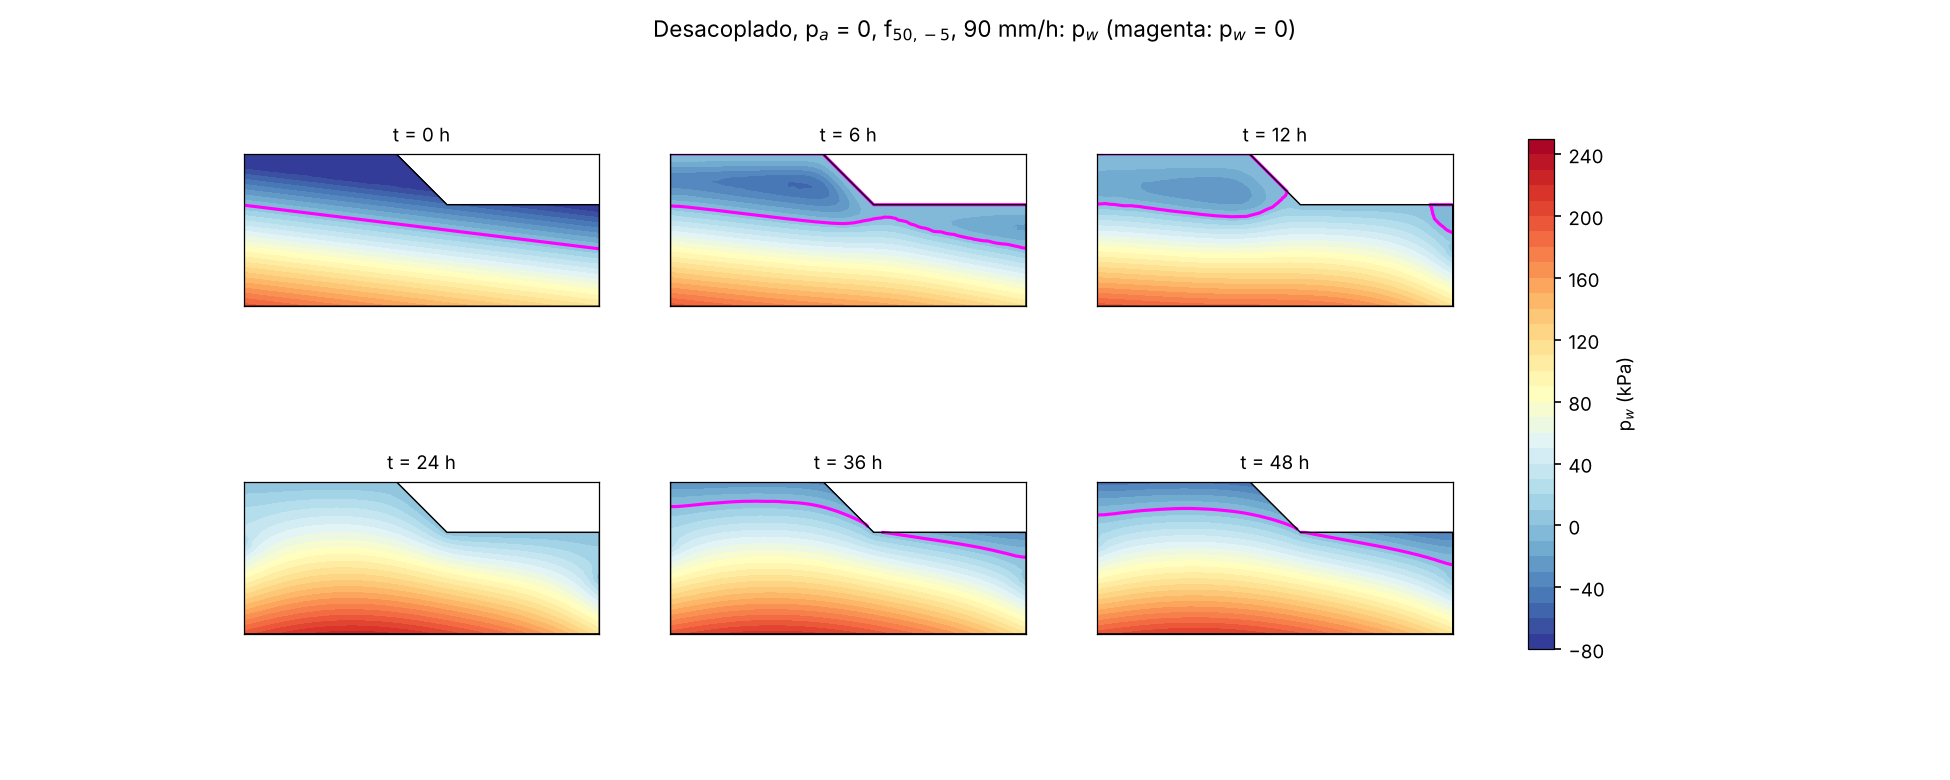
\includegraphics[width=0.95\textwidth]{figuras/campos_pw_f50_a45_H10_Hw5_I90_B_passivo_desacoplado.png}
\caption{Campos de press\~ao. Acima e no meio: modelo completo, $f_{50,-5}$, 36~mm/h ($p_w$ e $p_a$); o ar
pressurizado sob a frente de umedecimento torna $p_w$ positiva perto da superf\'icie. Abaixo: desacoplado com ar
passivo, 90~mm/h: eleva\c{c}\~ao do len\c{c}ol fre\'atico at\'e a face (categoria I/II da Tabela~3 do artigo).}
\label{fig:campos}
\end{figure}

\subsection{S\'erie A: \^angulo do talude}

A Tabela~7 do artigo n\~ao reproduz a pr\'opria Fig.~9 em algumas linhas (por exemplo, $f_{10}$ com 80~mm/h:
$2{,}830-0{,}027\cdot26{,}6=2{,}11$ na tabela e $\approx1{,}45$ na figura). A compara\c{c}\~ao usa os pontos lidos da
Fig.~9 ($\pm0{,}05$), Tabela~\ref{tab:A} e Fig.~\ref{fig:A}.

\begin{table}[htbp]
\centering
\caption{S\'erie A: FS m\'inimo, NeoPZ (modelo completo) / Fig.~9, para $\alpha=26{,}6$; 33,7; 45 e $63{,}4^\circ$.}
\label{tab:A}
\begin{tabular}{llcccc}
\toprule
Solo & $I_r$ (mm/h) & $26{,}6^\circ$ & $33{,}7^\circ$ & $45^\circ$ & $63{,}4^\circ$\\
\midrule
$f_{10,-4}$ & 9 & 2,37 / 2,35 & 2,17 / 2,16 & 1,93 / 1,88 & 1,60 / 1,45\\
 & 80 & 1,51 / 1,45 & 1,37 / 1,32 & 1,19 / 1,12 & 1,00 / 0,83\\
 & 360 & 1,21 / 1,15 & 1,07 / 1,00 & 0,99 / 0,82 & 0,99 / 0,62\\
$f_{50,-5}$ & 9 & 2,14 / 2,27 & 1,96 / 2,07 & 1,74 / 1,79 & 1,46 / 1,36\\
 & 36 & 1,34 / 1,43 & 1,16 / 1,27 & 1,01 / 1,04 & 0,74 / 0,76\\
 & 80 & 1,33 / 1,15 & 1,15 / 1,00 & 1,00 / 0,82 & 1,00 / 0,67\\
$f_{100,-6}$ & 3,6 & 2,18 / 2,37 & 1,99 / 2,19 & 1,77 / 1,89 & 1,49 / 1,45\\
 & 9 & 1,84 / 2,12 & 1,61 / 1,92 & 1,36 / 1,55 & 1,17 / 1,11\\
 & 80 & 1,77 / 2,05 & 1,53 / 1,83 & 1,27 / 1,45 & 1,01 / 1,05\\
\bottomrule
\end{tabular}
\end{table}

\begin{figure}[htbp]
\centering
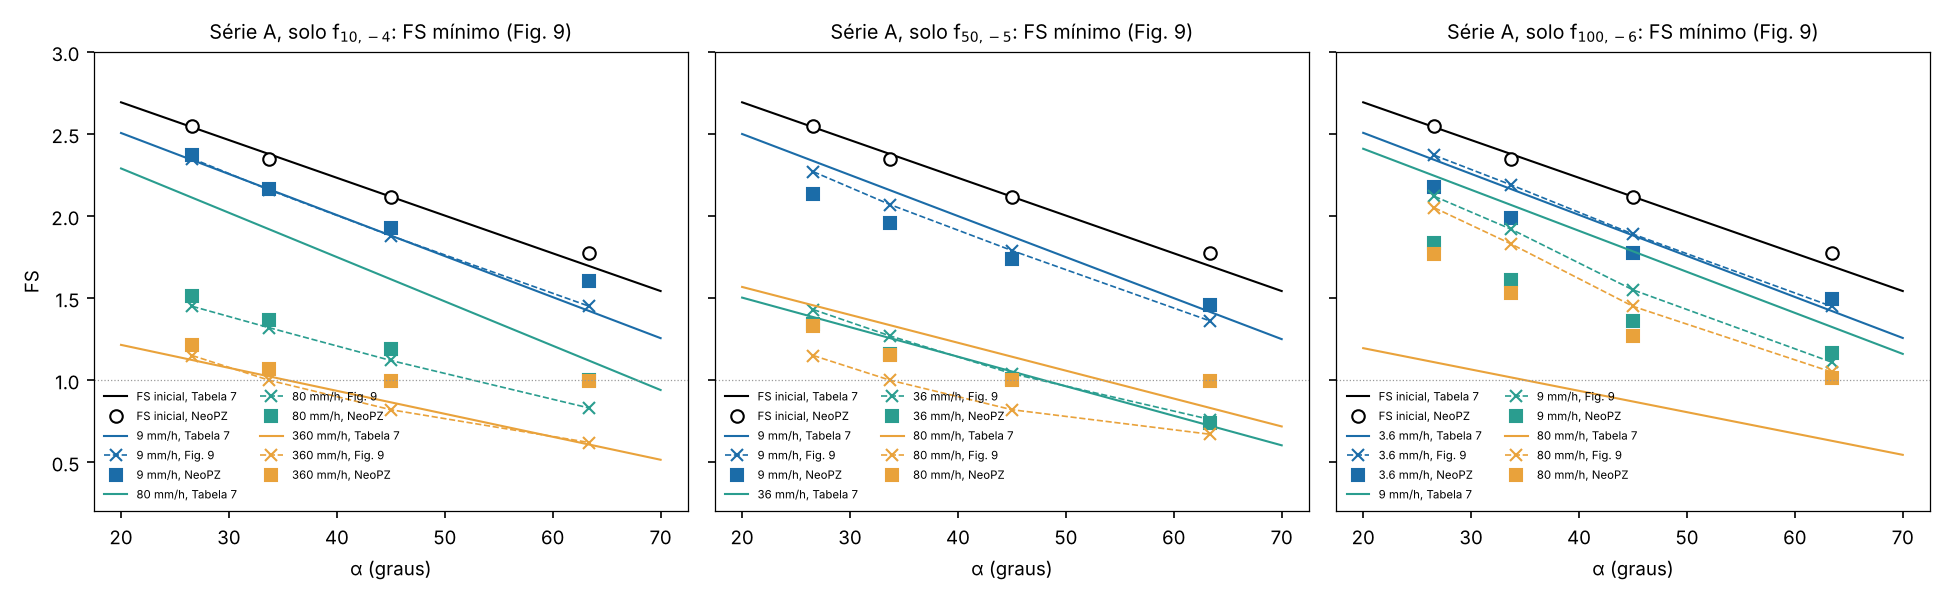
\includegraphics[width=\textwidth]{figuras/A_fs_min_alpha.png}
\caption{S\'erie A: FS inicial e m\'inimo $\times$ $\alpha$; linhas: Tabela~7; $\times$: Fig.~9; quadrados: NeoPZ.}
\label{fig:A}
\end{figure}

\begin{figure}[htbp]
\centering
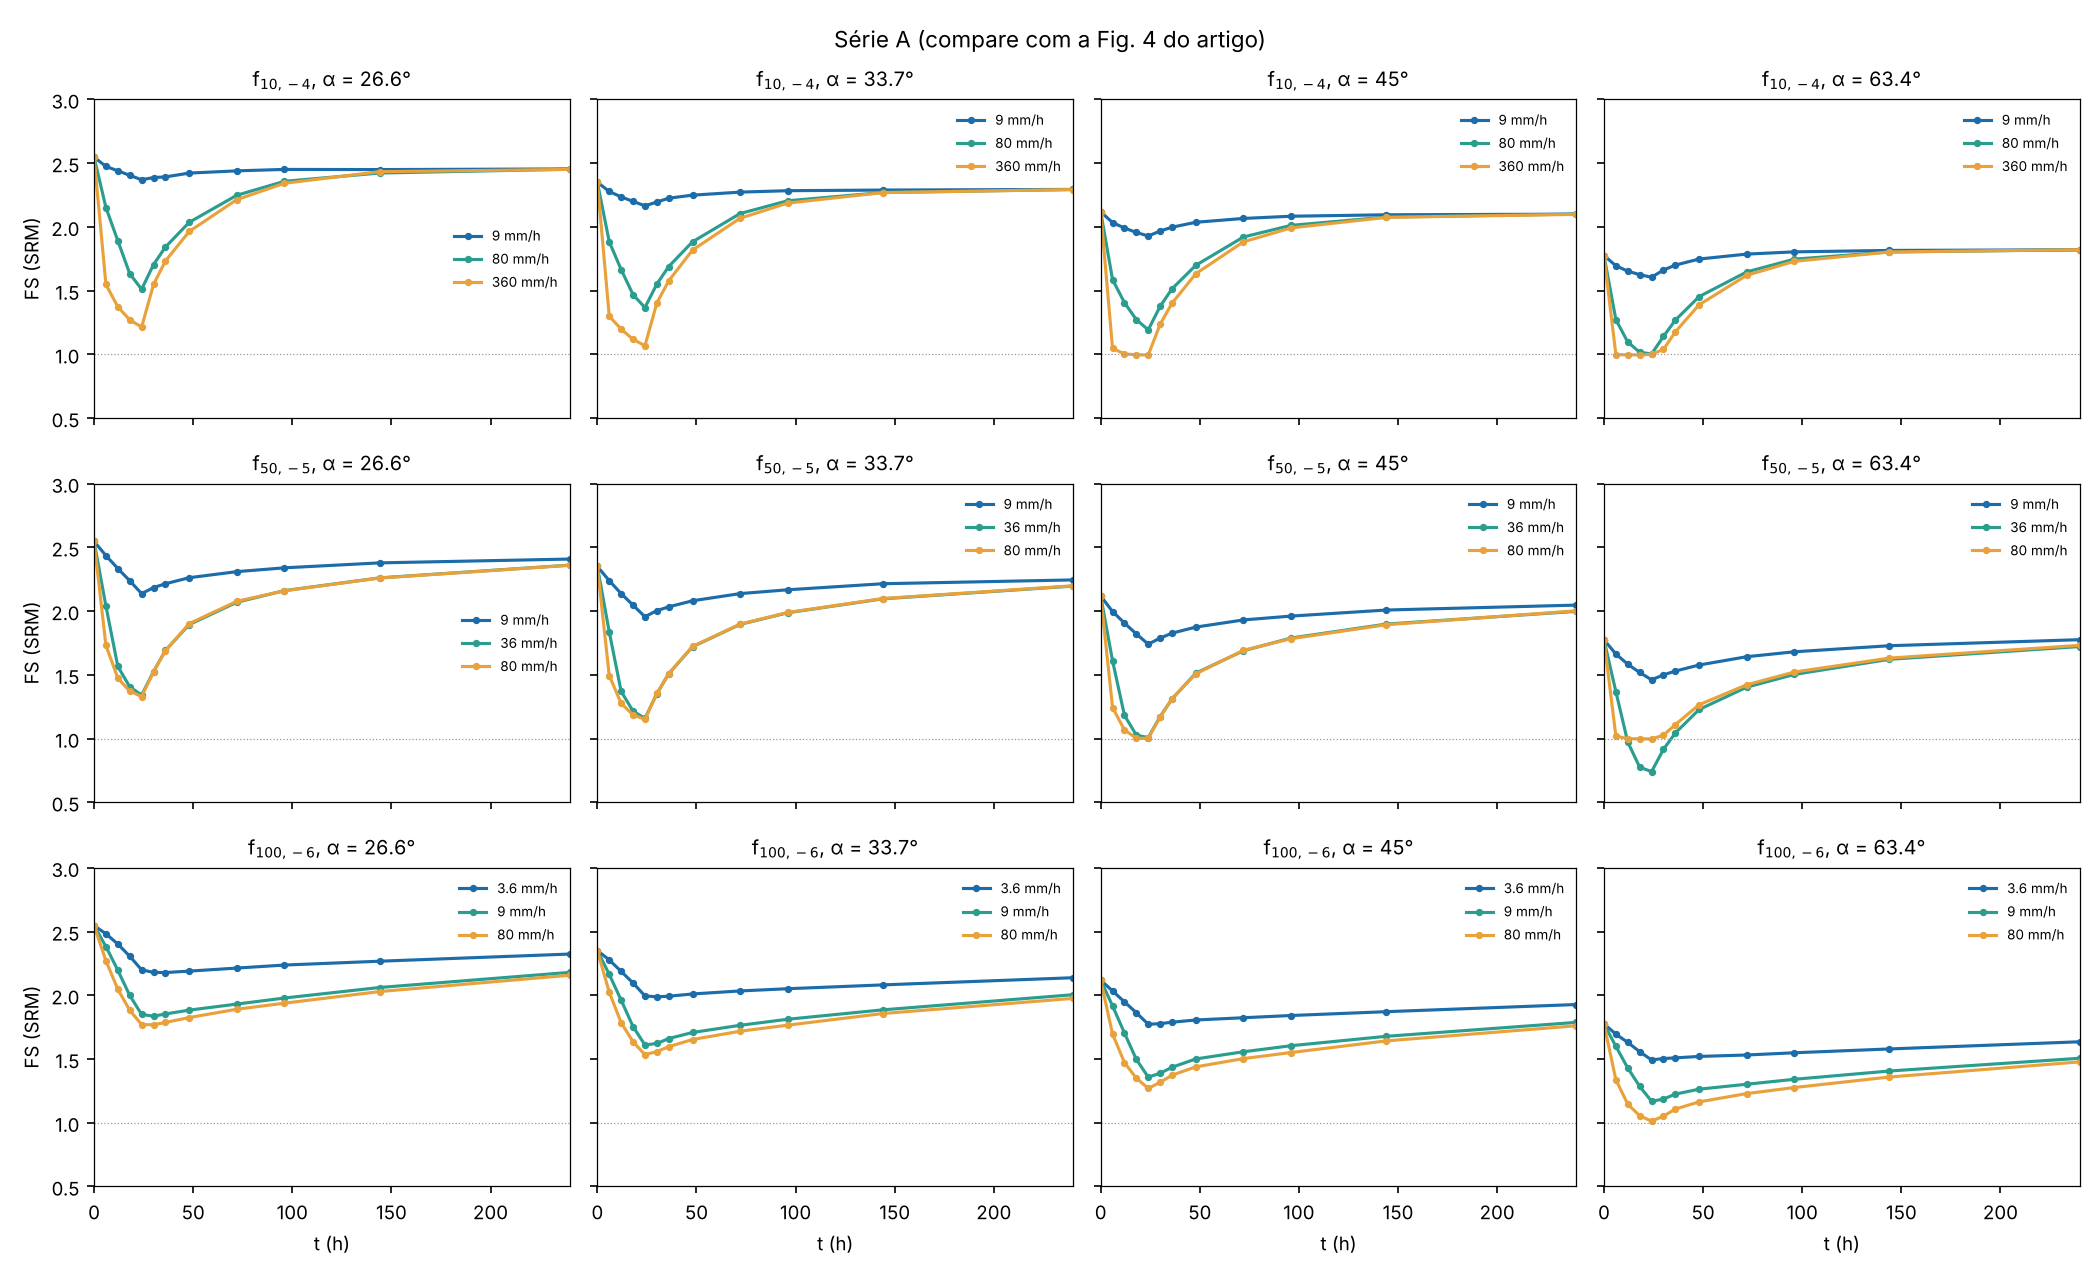
\includegraphics[width=\textwidth]{figuras/A_fs_tempo.png}
\caption{S\'erie A: FS($t$) at\'e 240~h (compare com a Fig.~4 do artigo).}\label{fig:A4}
\end{figure}

Nas chuvas fracas e moderadas o FS m\'inimo fica sobre a Fig.~9 (diferen\c{c}as at\'e 0,1, maiores no $f_{100}$, onde o
ar ativo reduz o FS); nas chuvas fortes aparece o patamar $\approx1$ do modelo acoplado. A diminui\c{c}\~ao do FS com
$\alpha$ \'e reproduzida: com 36~mm/h no $f_{50}$ o talude a $63{,}4^\circ$ rompe (0,74 contra 0,76; o transiente
perde o equil\'ibrio em $t=8$~h).

\subsection{S\'eries C e D: len\c{c}ol fre\'atico e altura}

\begin{table}[htbp]
\centering
\caption{S\'eries C e D: FS m\'inimo, NeoPZ (modelo completo) / Figs.~8 e 10.}\label{tab:CD}
\begin{tabular}{lccccc}
\toprule
S\'erie C, $H_w$ & 2,5~m & 5~m & 7,5~m & 10~m & 15~m\\
\midrule
9 mm/h & 1,38 / 1,43 & 1,74 / 1,79 & 2,01 / 2,00 & 2,17 / 2,13 & 2,31 / 2,20\\
36 mm/h & 1,00 / 0,85 & 1,00 / 1,04 & 1,03 / 1,19 & 1,08 / 1,26 & 1,14 / 1,29\\
80 mm/h & 1,00 / 0,81 & 1,00 / 0,82 & 1,01 / 1,05 & 1,04 / 1,15 & 1,09 / 1,16\\
\midrule
S\'erie D, $H_s$ & 5~m & 10~m & 20~m & 40~m & \\
\midrule
9 mm/h & 2,38 / 2,48 & 1,74 / 1,79 & 1,32 / 1,37 & 1,07 / 1,08 & \\
36 mm/h & 1,33 / 1,20 & 1,00 / 1,04 & 0,86 / 0,97 & 1,00 / 0,90 & \\
80 mm/h & 1,33 / 1,19 & 1,00 / 0,82 & 0,99 / 0,88 & 0,99 / 0,83 & \\
\bottomrule
\end{tabular}
\end{table}

\begin{figure}[htbp]
\centering
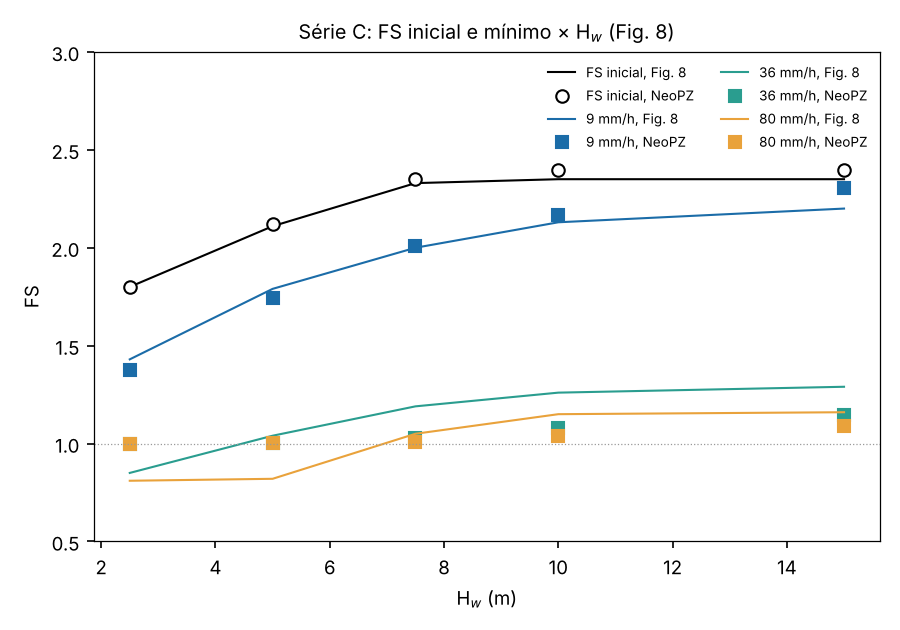
\includegraphics[width=0.49\textwidth]{figuras/C_fs_hw.png}\hfill
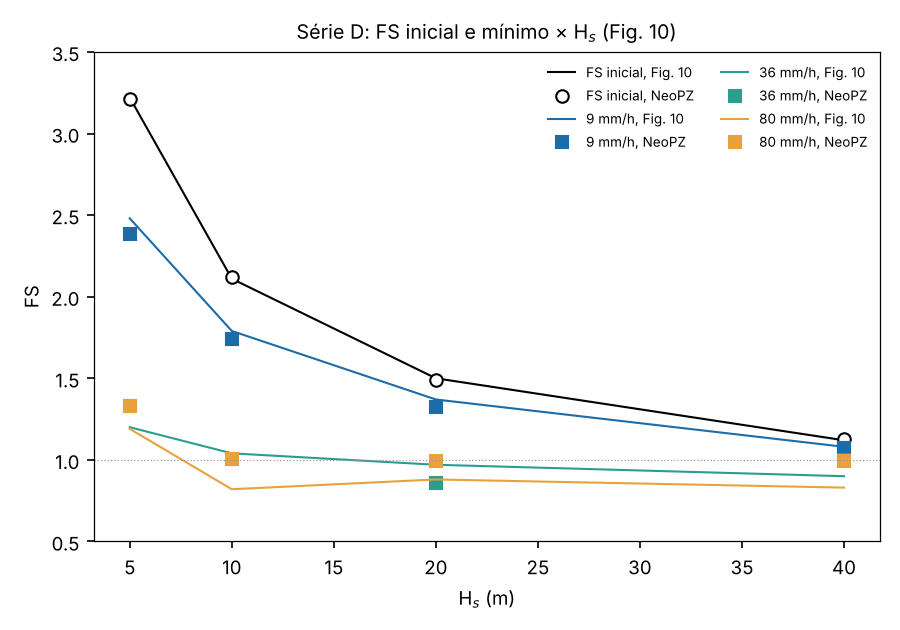
\includegraphics[width=0.49\textwidth]{figuras/D_fs_hs.png}
\caption{S\'eries C (esquerda, Fig.~8) e D (direita, Fig.~10): FS inicial e m\'inimo.}\label{fig:CD}
\end{figure}

Com 9~mm/h as S\'eries C e D reproduzem as Figs.~8 e 10 (diferen\c{c}as $\le0{,}11$). Nas chuvas de 36 e 80~mm/h o
FS do modelo acoplado volta ao patamar $\approx1$; os casos com $H_s=5$~m ficam acima do artigo (1,33 contra 1,20)
e o de 20~m com 36~mm/h abaixo (0,86 contra 0,97).

\subsection{Anisotropia da permeabilidade}

Solo $f_{50,-5}$, $\alpha=45^\circ$, $H_s=10$~m, $H_w=5$~m, 36~mm/h ($=k_s$) durante 24~h, modelo completo; o caso
isotr\'opico tem FS m\'inimo 1,005 (Tabelas~\ref{tab:aniso} e \ref{tab:rot}, Figs.~\ref{fig:aniso} e \ref{fig:rot}).

\begin{table}[htbp]
\centering
\caption{Tensor diagonal: FS m\'inimo e volume infiltrado em 24~h.}\label{tab:aniso}
\begin{tabular}{cccccc}
\toprule
$k_x$ (m/s) & $k_y$ (m/s) & $k_x/k_y$ & FS m\'in SRM & FS m\'in GI & infiltra\c{c}\~ao (m$^3$/m)\\
\midrule
$10^{-5}$ & $10^{-5}$ & 1 & 1,005 & 1,01 & 38,4\\
$3\cdot10^{-5}$ & $10^{-5}$ & 3 & 1,035 & 1,10 & 40,2\\
$10^{-4}$ & $10^{-5}$ & 10 & 1,078 & 1,25 & 42,7\\
$10^{-5}$ & $10^{-6}$ & 10 & 1,259 & 1,75 & 16,0\\
$10^{-6}$ & $10^{-5}$ & 0,1 & 1,002 & 1,01 & 35,5\\
$10^{-5}$ & $10^{-4}$ & 0,1 & 1,195 & 1,56 & 53,9\\
\bottomrule
\end{tabular}
\end{table}

\begin{table}[htbp]
\centering
\caption{Tensor girado: $k_1=10^{-4}$~m/s na dire\c{c}\~ao $\theta$, $k_2=10^{-5}$~m/s normal a ela. A face desce a
$-45^\circ$: $\theta=135^\circ$ \'e a dire\c{c}\~ao da face.}\label{tab:rot}
\setlength{\tabcolsep}{4pt}
\begin{tabular}{lcccccccccccc}
\toprule
$\theta$ ($^\circ$) & 0 & 15 & 30 & 45 & 60 & 75 & 90 & 105 & 120 & 135 & 150 & 165\\
\midrule
FS m\'in SRM & 1,08 & 1,19 & 1,33 & 1,33 & 1,28 & 1,24 & 1,20 & 1,16 & 1,15 & 1,18 & 1,20 & 1,11\\
FS m\'in GI & 1,24 & 1,64 & 2,21 & 2,16 & 1,95 & 1,73 & 1,55 & 1,42 & 1,37 & 1,49 & 1,60 & 1,36\\
Infiltra\c{c}\~ao (m$^3$/m) & 43,0 & 48,1 & 52,9 & 53,8 & 53,7 & 53,7 & 53,9 & 54,8 & 56,3 & 57,9 & 57,3 & 50,0\\
\bottomrule
\end{tabular}
\end{table}

\begin{figure}[htbp]
\centering
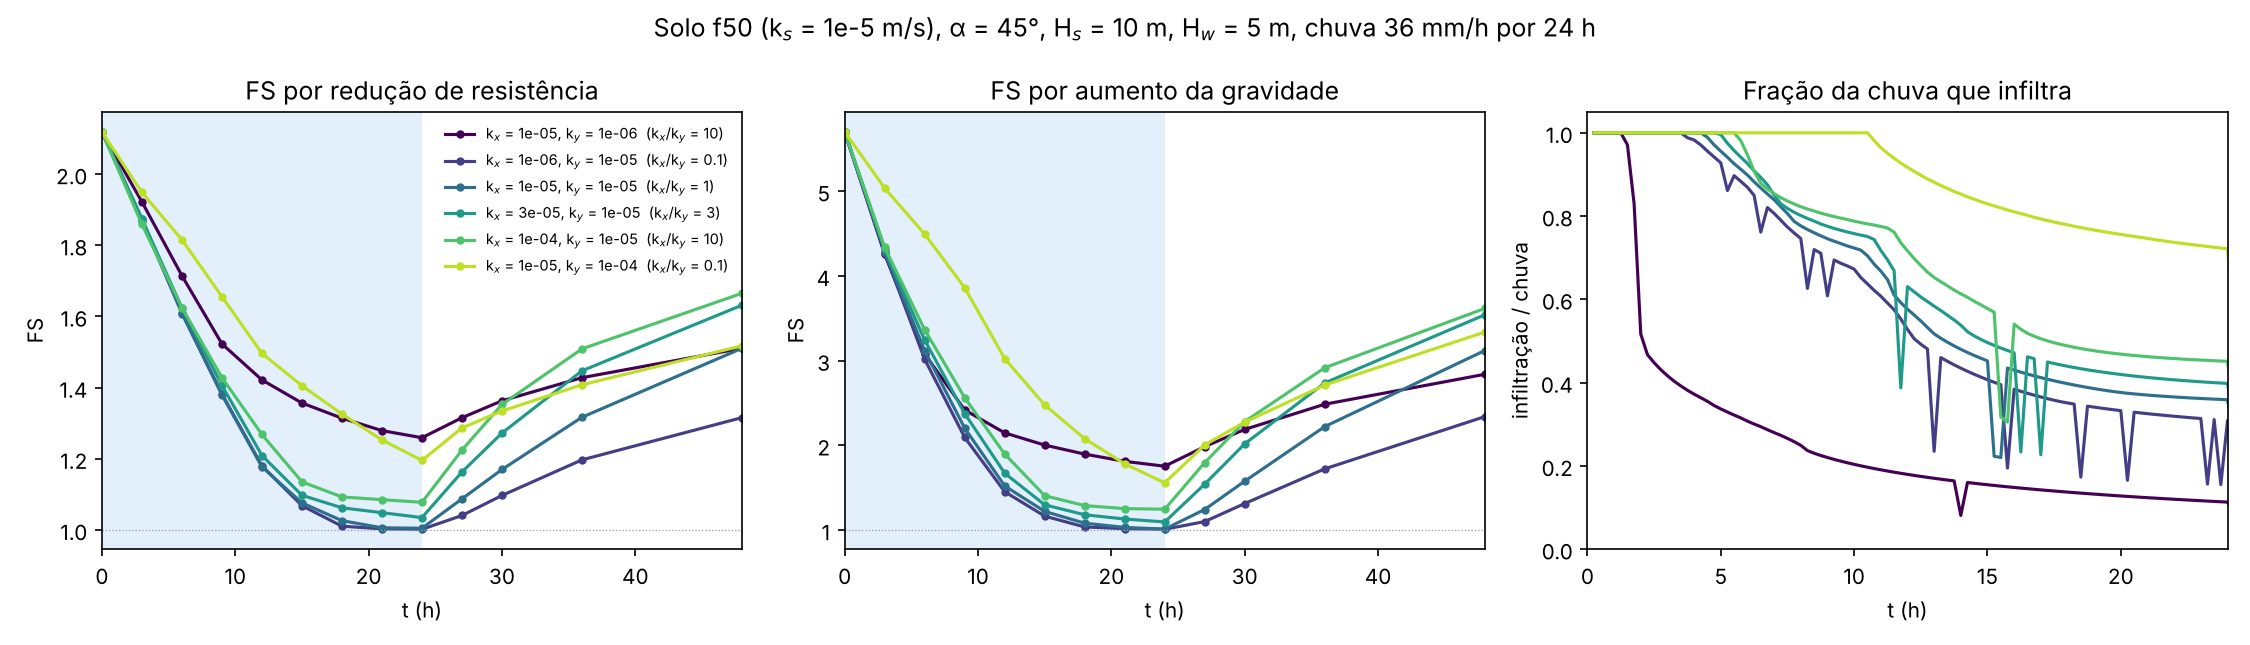
\includegraphics[width=\textwidth]{figuras/anisotropia_fs.png}
\caption{Tensor diagonal: FS($t$) por redu\c{c}\~ao de resist\^encia e por aumento da gravidade, e fra\c{c}\~ao da chuva
que infiltra.}\label{fig:aniso}
\end{figure}

\begin{figure}[htbp]
\centering
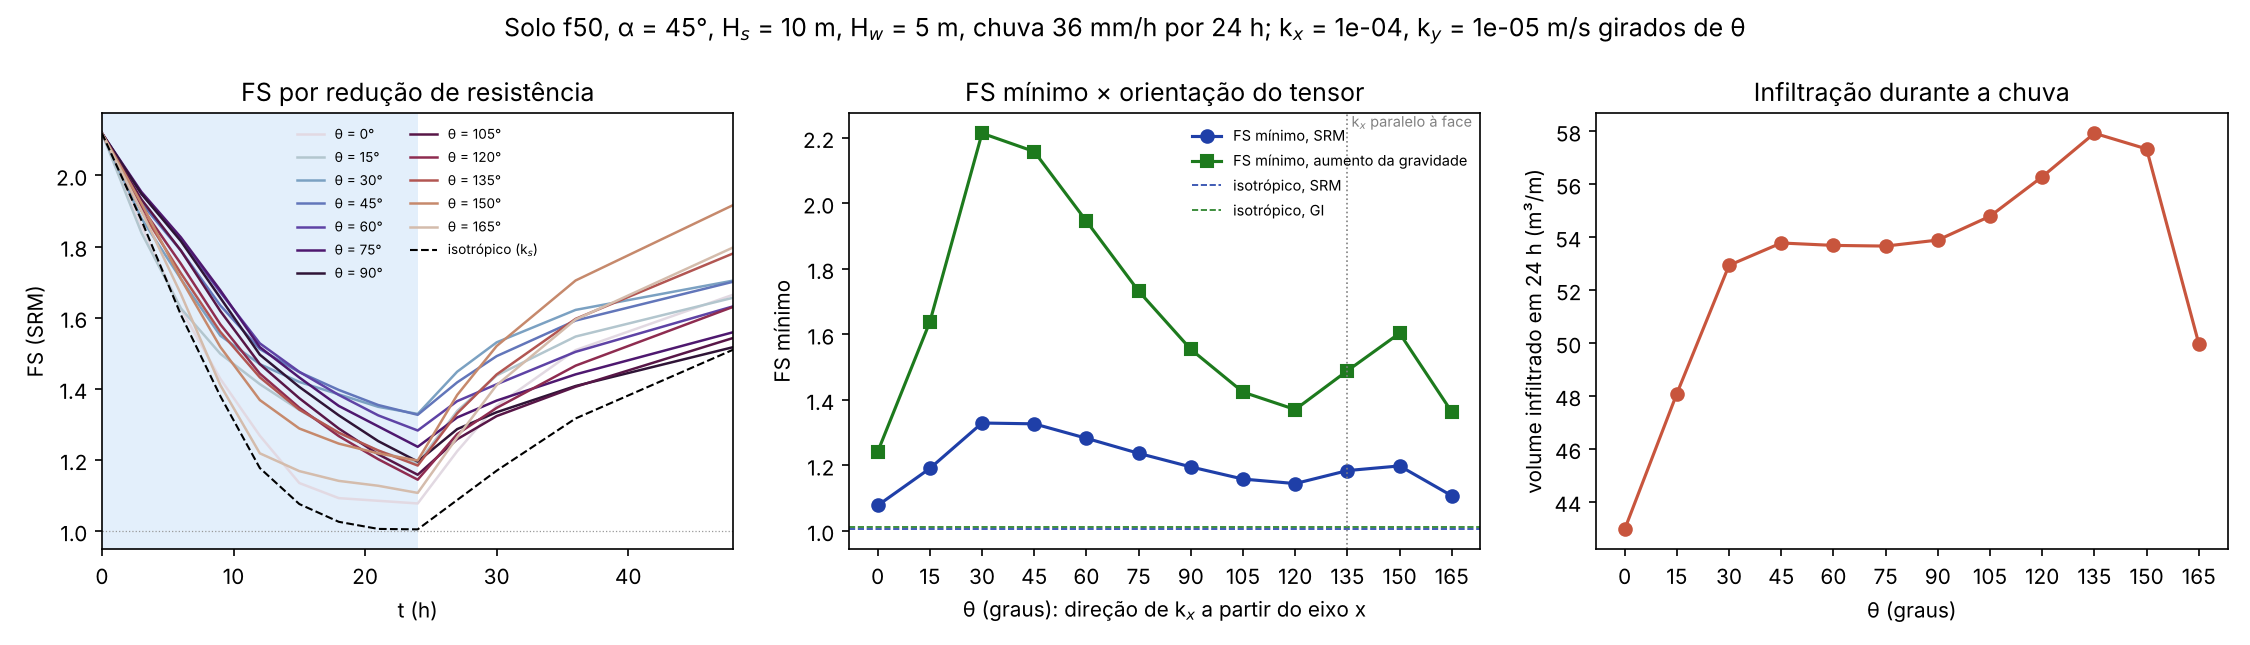
\includegraphics[width=\textwidth]{figuras/rotacao_fs.png}
\caption{Tensor girado de $15^\circ$ em $15^\circ$: FS($t$), FS m\'inimo $\times$ $\theta$ e infiltra\c{c}\~ao.}
\label{fig:rot}
\end{figure}

\begin{itemize}
\item Com $k_y<k_s$ a chuva infiltra menos (escoa na superf\'icie) e o FS sobe (1,26); com $k_x>k_y$ a \'agua se
espalha lateralmente e drena pela face.
\item Com $k_y>k_x$ infiltra mais \'agua (53,9 m$^3$/m), mas o FS tamb\'em sobe (1,20): a frente desce r\'apido e
drena, sem saturar a zona rasa.
\item Girando o tensor, o pior caso \'e $\theta=0$ (estratifica\c{c}\~ao horizontal) e o melhor $\theta\approx30$--$45^\circ$
(dire\c{c}\~ao mais perme\'avel subindo para dentro do maci\c{c}o, contr\'aria \`a face): a \'agua \'e conduzida para longe
da face. Todos os casos anisotr\'opicos ficam acima do isotr\'opico com o mesmo $k_{\min}=k_s$.
\end{itemize}

\subsection{P\'os-processamento}

Para cada caso, o script \texttt{animacao.py} (ou \texttt{mma/animacao.wl} no Mathematica) gera o FS em escala
$\log t$ (Fig.~\ref{fig:fstempo}; $t=0$ desenhado em 0,01~h, linha vertical no instante de ruptura do transiente) e
uma anima\c{c}\~ao das isolinhas de $p_w$ (preenchimento a cada 10~kPa, isolinhas rotuladas a cada 50~kPa, $p_w=0$
em magenta) ao lado do gr\'afico do FS, com o marcador do instante interpolado linearmente em $\log t$.

\begin{figure}[htbp]
\centering
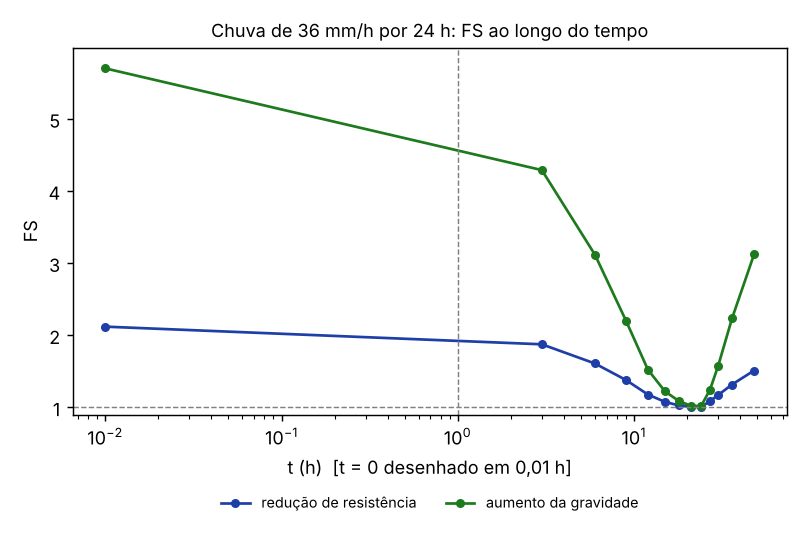
\includegraphics[width=0.48\textwidth]{figuras/fs_tempo_f50_I36.png}\hfill
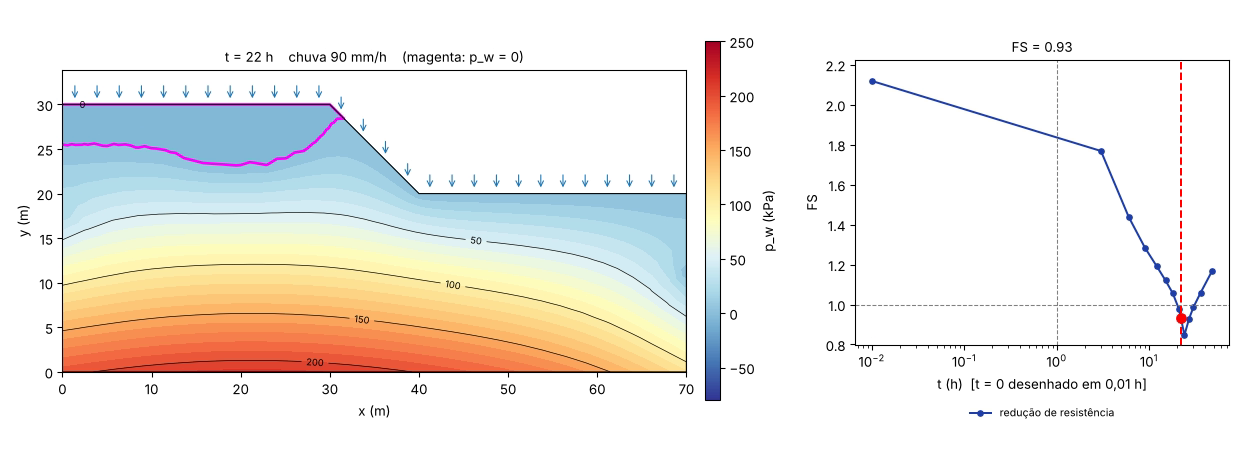
\includegraphics[width=0.50\textwidth]{figuras/quadro_animacao_f50_I90.png}
\caption{Esquerda: FS($t$) em escala log, modelo completo, $f_{50,-5}$, 36~mm/h (SRM e GI). Direita: quadro da
anima\c{c}\~ao (desacoplado, 90~mm/h, $t=22$~h).}\label{fig:fstempo}
\end{figure}

%======================================================================
\section{Contraexemplos \`as conclus\~oes de Rahardjo et al.\ (2007)}\label{sec:contraexemplos}
%======================================================================

As conclus\~oes do artigo foram obtidas com percola\c{c}\~ao desacoplada, ar passivo, solo isotr\'opico, $\chi=1$,
suc\c{c}\~ao inicial limitada a 75~kPa e equil\'ibrio-limite com superf\'icies circulares. O modelo desta nota permite
relaxar cada uma dessas hip\'oteses. Os itens abaixo s\~ao hip\'oteses de investiga\c{c}\~ao que podem contradizer
(ou restringir) as conclus\~oes do artigo; para cada um indicam-se a evid\^encia j\'a obtida e o teste proposto.

\subsection{A1. O patamar de FS m\'inimo (``intensidade-limite'') depende da dilat\^ancia}

\textbf{Conclus\~ao do artigo:} existe uma intensidade $I_{r(\mathrm{thr})}$ acima da qual o FS m\'inimo n\~ao diminui,
com patamar inferior 0,81--0,82 (Eq.~6, Fig.~7).

\textbf{Evid\^encia:} desacoplado, o NeoPZ reproduz o patamar (0,84--0,86); acoplado, o patamar sobe para
$\approx1{,}00$ e o transiente nunca perde o equil\'ibrio (Tabela~\ref{tab:B}). O mecanismo proposto \'e a suc\c{c}\~ao
gerada pela dilat\^ancia pl\'astica ($\psi=\phi'$) na percola\c{c}\~ao acoplada.

\textbf{Teste:} repetir a S\'erie B acoplada com $\psi=0$, $\phi'/2$ e $\phi'$. Se o patamar descer de 1,00 a 0,82
quando $\psi\to0$, a ``intensidade-limite com FS $<1$'' depende de uma hip\'otese constitutiva n\~ao discutida no
artigo, e a an\'alise desacoplada \'e conservadora apenas para solos contrativos. \emph{Requer} um Mohr--Coulomb
n\~ao associativo (o retorno anal\'itico atual exige $\psi=\phi'$; alternativa: \texttt{TPZPlasticStepPV}).

\subsection{A2. ``Taludes pouco perme\'aveis s\~ao seguros em chuvas curtas''}

\textbf{Conclus\~ao do artigo:} solos com $k_s\le10^{-6}$~m/s n\~ao rompem em chuvas de at\'e 24~h, qualquer que seja a
intensidade (categoria IV, sem eleva\c{c}\~ao do NA).

\textbf{Evid\^encia:} com ar ativo o FS m\'inimo do $f_{100}$ cai de 1,50 (ar passivo) para 1,28 com 18~mm/h e
de 1,48 para 1,28 com 36~mm/h (Tabela~\ref{tab:B}), ficando abaixo da Eq.~6 (1,45); o ar aprisionado chega a
50~kPa e torna $p_w$ positiva sob a frente (Fig.~\ref{fig:campos}). Na S\'erie A, com ar ativo, o $f_{100}$ com
80~mm/h chega a 1,01 em $\alpha=63{,}4^\circ$.

\textbf{Teste:} $f_{100}$ com $\alpha=63{,}4^\circ$ e $H_s=20$~m, chuvas de 9 a 80~mm/h, com e sem ar ativo, e
$k_{ra}^{\min}$ variando de $10^{-6}$ a $10^{-2}$ (a sa\'ida do ar controla a pressuriza\c{c}\~ao). Um FS $<1$ apenas
com ar ativo seria um contraexemplo direto. N\~ao requer c\'odigo novo.

\subsection{A3. ``O controle \'e $k_s$'': com anisotropia $k_s$ n\~ao \'e um n\'umero}

\textbf{Conclus\~ao do artigo:} $I_{r(\mathrm{ini})}$ e $I_{r(\mathrm{thr})}$ s\~ao dados em m\'ultiplos de $k_s$
($0{,}03$--$0{,}78k_s$ e $0{,}39$--$3k_s$, Fig.~7).

\textbf{Evid\^encia:} mesmo solo, mesma chuva e o mesmo $k_{\min}$, s\'o girando o tensor: FS m\'inimo de 1,08 a 1,33
(Tabela~\ref{tab:rot}); com $k_x/k_y=10$, FS de 1,08 ou 1,26 conforme qual componente vale $k_s$.

\textbf{Teste:} curvas FS m\'inimo $\times$ $I_r$ (S\'erie B) para $k_1/k_2=10$ e $\theta=0$, $45^\circ$ e $135^\circ$,
verificando se a sigmoide se desloca com $k_y$, com a condutividade normal \`a superf\'icie, com a condutividade ao
longo da face ou com $\sqrt{k_1k_2}$. N\~ao requer c\'odigo novo ($\approx20$ casos).

\subsection{A4. ``O len\c{c}ol fre\'atico inicial \'e secund\'ario'': efeito do limite de suc\c{c}\~ao}

\textbf{Conclus\~ao do artigo:} $H_w$ s\'o define o FS inicial; o pr\'oprio artigo nota que o FS inicial deixa de
crescer acima de $H_w=7{,}5$~m por causa do limite de $-75$~kPa (Fig.~8).

\textbf{Teste:} S\'erie C com suc\c{c}\~ao inicial limitada a 75, 150 e 300~kPa e sem limite. Se a queda de FS
(FS inicial $-$ FS m\'inimo) passar a depender fortemente de $H_w$, o car\'ater ``secund\'ario'' do NA \'e artefato do
limite. \emph{Requer} tornar o limite (\texttt{SMAX}) um par\^ametro.

\subsection{A5. ``O FS m\'inimo \'e linear em $\alpha$ com inclina\c{c}\~ao quase constante''}

\textbf{Conclus\~ao do artigo:} $F_{s(\min)}=E+F\alpha$ com $F\approx-0{,}025$ (Tabela~7).

\textbf{Evid\^encia:} a Tabela~7 n\~ao reproduz a Fig.~9 em algumas linhas; com quatro \^angulos a linearidade n\~ao
\'e test\'avel. No NeoPZ a inclina\c{c}\~ao muda nas chuvas fortes por causa do patamar $\approx1$.

\textbf{Teste:} $\alpha$ de $20^\circ$ a $70^\circ$ a cada $5^\circ$ para os nove pares solo--chuva, observando
tamb\'em a profundidade do mecanismo (zona pl\'astica rasa $\times$ profunda). N\~ao requer c\'odigo novo.

\subsection{A6. Intensidade ou volume?}

\textbf{Conclus\~ao do artigo:} $I_r=1k_s$ n\~ao produz necessariamente o menor FS; o volume $V_r$ \'e citado, mas
todas as chuvas t\^em 24~h.

\textbf{Teste:} chuvas com o mesmo volume e dura\c{c}\~oes de 3, 6, 24 e 72~h. Se o FS m\'inimo depender s\'o do volume
para solos de alto $k_s$ e s\'o da intensidade para solos de baixo $k_s$, a conclus\~ao precisa ser reformulada. N\~ao
requer c\'odigo novo (par\^ametro \texttt{train}).

%======================================================================
\section{Novas dire\c{c}\~oes}\label{sec:direcoes}
%======================================================================

\subsection{B1. Defini\c{c}\~ao do fator de seguran\c{c}a com suc\c{c}\~ao}

O FS por aumento da gravidade \'e 5,7 contra 2,1 do SRM no estado inicial e varia muito mais com a orienta\c{c}\~ao do
tensor (1,24--2,21 contra 1,08--1,33). Proposta: comparar SRM, GI e Bishop simplificado nos mesmos campos de press\~ao
e verificar se o SRM detecta rupturas rasas na frente de umedecimento (transla\c{c}\~ao) que a superf\'icie circular de
Bishop n\~ao representa.

\subsection{B2. Par\^ametro de Bishop}

O artigo usa $\phi^b=\phi'$ ($\chi=1$). Com $\chi=S_w$ (j\'a dispon\'ivel no material) ou $\phi^b<\phi'$, a perda de
suc\c{c}\~ao pesa menos e o mecanismo atribu\'ido aos solos pouco perme\'aveis enfraquece; a tangente com
$\chi_w=S_w-\Gamma p_c$ (Se\c{c}\~ao 13.4) torna o acoplamento n\~ao sim\'etrico.

\subsection{B3. Chuva antecedente e padr\~ao temporal}

Duas chuvas separadas por intervalos secos e padr\~oes adiantado, atrasado e uniforme com o mesmo total. O artigo
afirma qualitativamente que a chuva antecedente importa para baixo $k_s$; no $f_{100}$ o m\'inimo j\'a ocorre depois
do fim da chuva ($t=27$~h). \emph{Requer} intensidade vari\'avel no tempo.

\subsection{B4. Tratamento da superf\'icie}

O artigo imp\~oe $q=I_r$; aqui a condi\c{c}\~ao \'e unilateral (escoamento superficial quando $p_w$ atinge 0). Rodar as
duas condi\c{c}\~oes isola quanto do patamar e da intensidade-limite vem do tratamento da superf\'icie.

\subsection{B5. F\'isica prevista na formula\c{c}\~ao e ainda n\~ao usada}

\begin{itemize}
\item histerese da curva de reten\c{c}\~ao (secagem $\times$ umedecimento), que deve afetar a recupera\c{c}\~ao depois da
chuva;
\item porosidade vari\'avel (Se\c{c}\~ao 9) e reten\c{c}\~ao dependente da porosidade (Se\c{c}\~ao 11) com
Kozeny--Carman;
\item evapora\c{c}\~ao e transpira\c{c}\~ao como fluxo negativo (Fig.~1 do artigo);
\item varia\c{c}\~ao espacial de $k_s$ e $c'$ (campos aleat\'orios), na linha de Ceron et al.\ (2025).
\end{itemize}

\subsection{Prioridades}

\begin{enumerate}
\item A2 (ar ativo em solo pouco perme\'avel): contraexemplo mais direto, sem c\'odigo novo.
\item A3 (anisotropia na sigmoide de $I_r$): usa o que foi implementado e pode gerar um resultado original.
\item A1 (dilat\^ancia): explica a diferen\c{c}a entre o modelo acoplado e o artigo; requer Mohr--Coulomb n\~ao
associativo.
\end{enumerate}

\subsection{Limita\c{c}\~oes dos resultados atuais}

\begin{itemize}
\item Em dois casos acoplados um passo n\~ao converge nem com 5 bissec\c{c}\~oes (FS $\approx1{,}8$--$1{,}9$); o instante \'e
registrado como ``transiente sem converg\^encia'', n\~ao como ruptura.
\item Na variante desacoplada, $f_{10}$ com 360 e 900~mm/h: a percola\c{c}\~ao parou de convergir \`as 8,5~h com toda a
superf\'icie alagada; o m\'inimo est\'a superestimado.
\item FS por elementos finitos (SRM) e n\~ao por equil\'ibrio-limite; porosidade constante; sem histerese; uma \'unica
malha (sem estudo de converg\^encia).
\end{itemize}
